\documentclass[11pt,a4paper]{article}
%\usepackage[toc,page]{appendix}
\usepackage{graphicx}
\usepackage[a4paper]{geometry}
\usepackage{xcolor}
\usepackage{fancyhdr}
\usepackage{float}
\usepackage{setspace}
\usepackage[absolute]{textpos}
\usepackage{epstopdf}
%\usepackage[]{mcode} 	% To include matlab code
\usepackage{capt-of}
\usepackage{enumerate}
\usepackage{lastpage}
\usepackage{booktabs}
\usepackage{longtable}
\usepackage{array}
\renewcommand{\arraystretch}{1.5}

\usepackage[english]{babel}
\usepackage[utf8]{inputenc}
\usepackage{amsmath}
\usepackage{amsfonts}
\usepackage{graphicx}
\usepackage[colorinlistoftodos]{todonotes}
\usepackage{algorithm}
\usepackage{algpseudocode}

\usepackage{amsmath}
\usepackage{algorithm}
%\usepackage[noend]{algpseudocode}
\makeatletter
\def\BState{\State\hskip-\ALG@thistlm}
\makeatother

\usepackage{amsmath}
\usepackage{amsfonts}
\usepackage{amssymb}
\usepackage{eurosym}

% Header
\setlength{\headheight}{30pt}
\newgeometry{top=2.5cm, bottom = 1.5cm, left=2cm, right=2cm}
\pagestyle{fancy} 
\lhead{\includegraphics[height=0.8cm]{figures/{tue_logo}.png}}
%\lfoot{Group 4 - ``CASE"-HENK}
\cfoot{~}
\rfoot{Page \thepage ~of \pageref{LastPage}}

\usepackage{cleveref}
% Change cleveref reference eq. to equation same for figure
\crefname{equation}{equation}{equations}
\crefname{figure}{figure}{figures}
\crefname{table}{table}{tables}

% Change Section numbering to Problem 1
%\renewcommand{\thesection}{Problem \arabic{section}.}

\begin{document}
%\begin{titlepage}
%\vspace*{100pt}
%\begin{figure}
%\centering
%\includegraphics[width=0.5\textwidth]{figures/TUelogozondertekst}
%\end{figure}
%\begin{center}
%{ \huge \bfseries 4AT100 Automotive Systems Engineering Project\\[0.4cm] }
%\textsc{\Large Concept Project Plan}\\[0.5cm]
%
%\end{center}
%
%\vfill
%
%\renewcommand{\arraystretch}{1}
%
%\begin{flushleft} \large
%\begin{tabular}{l}
%Project Coordinators:\\
%Dr.Ir. A. van de Mortel-Fronczak (Asia) \\
%Dr.Ir. I. Barosan (Ion) \\
%\end{tabular}
%\end{flushleft}
%
%\begin{flushleft} \large
%\begin{tabular}{l l l l}
%Tutor: & & & \\
%L. Kefalidis (Lazaros) & & & \\
%& & & \\
%Authors:\hspace{30mm} 	& \hspace{35mm}	& \hspace{55mm} 	    		& 			\\
%S. Forno (Simone) 		& ​0978942		& T. de Mor\'ee (Tim)			& 0944052 	\\
%R.M.A. Goris (Rob) 		& 0808822		& T.M.A. van de Wiel (Thijs)	​& 0824530 	\\
%B.S. Haarsma (Bouke) 	& 0751757​		& H. Wils (Hielke) 				& 0807014 	\\
%\end{tabular}
%\end{flushleft}
%
%\begin{flushleft} \large
%\begin{tabular}{l}
%MSc. Programme Automotive Technology \\
%Eindhoven University of Technology \\
%\end{tabular}
%\end{flushleft}
%
%\begin{flushleft} \large
%\begin{tabular}{l}
%\today \hspace{8.4cm} Group 4 ``CASE"-HENK \\
%\end{tabular}
%\end{flushleft}
%
%\renewcommand{\arraystretch}{1.5}
%
%\end{titlepage}

\newgeometry{top=2.5cm, bottom = 3cm, left=2cm, right=2cm}

%\newpage
%
%\setcounter{tocdepth}{2}
%
%\tableofcontents
%\newpage


%------------------------------------------------

\section{Background and scope of the work}
In this section I will briefly introduce the work´s background and the aim of the research.

Title of the work is "Implementation and comparison of methodologies for indoor self-localization of AMR", where the acronym AMR stands for Automated Mobile Robots. The referred methodologies are 2 localization algorithms (a Gmapping Particle Filter and a Feauture Based EKF), which the robot uses to retrieve its pose (in $x$, $y$, $\theta$ coordinates) and map the environment (i.e. reconstruct it) using the SLAM approach. SLAM stands for Self Localization and Mapping. To test the methods, the trajectory of Figure \ref{fig:traj} is used, which represents a standard docking-delivery trajectory. The AMR performance is calculate by the error deviation from a theoretical trajectory and the one the robot actually performs in the simulation, hence an error estimate. 

The "Montagelinie" of Figure \ref{fig:WZL_Layout} will be simulated as a rectangular sum of individual blocks representing individual stations. At the end of the Open Loop manouvre of Figure \ref{fig:traj}, the AMR stops in the middle of 2 stations.

For the simulation we use ROS Indigo on Ubuntu 14.04 and Gazebo 2.2 software, integrated with ROS.

\begin{figure}[!htb]
    \centering
    \begin{minipage}{.5\textwidth}
        \centering
        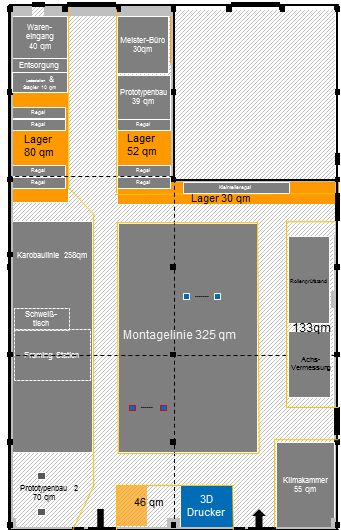
\includegraphics[width=0.7\linewidth, height=0.4\textheight]{figures/Layout_WZL}
        \caption{WZL production plant in Aachen}
        \label{fig:WZL_Layout}
    \end{minipage}%
    \begin{minipage}{0.5\textwidth}
        \centering
        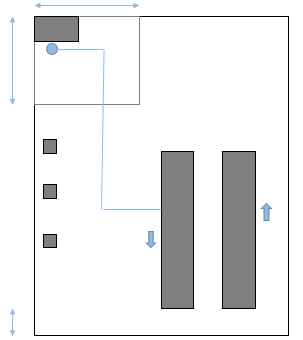
\includegraphics[width=0.6\linewidth, height=0.2\textheight]{figures/close_loop}
        \caption{Open Loop trajectory}
        \label{fig:traj}
    \end{minipage}
 \end{figure}

\section{Updates}

Before making the WZL site in Gazebo, the algorithm are tested in the $simple$ $indoor$ $environment$, according to the plan, found in the Prep. phase dedicated section. The first will be the Gmapping Particle Filter, which pseudocode is found in page 4. The simple indoor plant resambles the MRL Arena [1]. This small indoor environment contains an uneven structure, which is suitable to test the Gmapping or Amcl package algorithm already provided by the ROS distribution. The resulting building indoor environment is visible in Figure \ref{fig:MRL_arena} and Figure \ref{fig:2d_MRL}. The figure shows two extra white small blocks, which I will discuss later on. They represent a WirelessTransmitter and Receiver world model, needed to begin the Global Localiztion of the algorithm.

\begin{figure}[!htb]
    \centering
    \begin{minipage}{.5\textwidth}
        \centering
        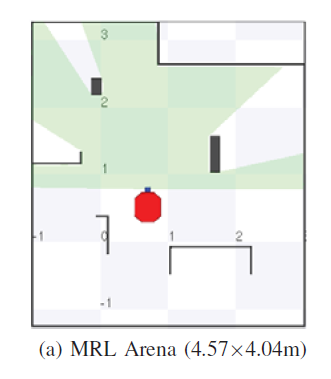
\includegraphics[width=0.7\linewidth, height=0.2\textheight]{figures/MRL2d_arena}
        \caption{The 2D model arena, used to reproduce the simple model arena}
        \label{fig:2d_MRL}
    \end{minipage}%
    \begin{minipage}{0.5\textwidth}
        \centering
        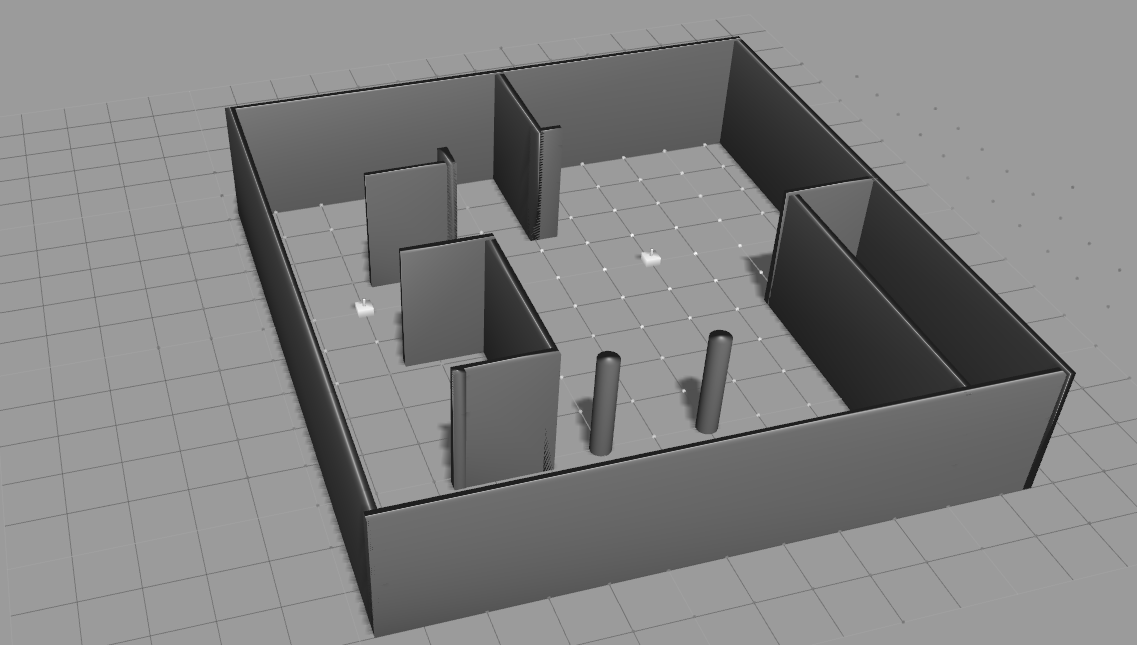
\includegraphics[width=1\linewidth, height=0.2\textheight]{figures/Gazebo_indoor}
        \caption{Realization of the model in Gazebo}
        \label{fig:MRL_arena}
    \end{minipage}
 \end{figure}

Each world defined in the Gazebo simulator consists of several components, whose characteristics are visible in Figure \ref{fig:small_indoor} and Figure \ref{fig:wireless_trans}. The world model is written in a XML fashion and includes collision, visual and inertial property. In this example the link for Wall18 is one of the component of the entire indoor arena, whose collision property defines the wall's dimension (and the obstructed space it covers in the world), the visual the visibility in the GUI, and the inertial the physical properties. Most of the times collision and visual coincide, like in this case. The only relevant $parameters$ for this static arena are the poses of the walls. By adding more "pieces", the entire indoor world has been created. 

The WirelessTransmitter (I will explain why this model has been added in the following part) model contains a further tag, the $sensor$ tag, which includes the plugin that fires the sensor to transmit data over the Gazebo simulator. It is actually not visible here the process that is is hidden behind, but by adding the $<plugin name: filename: .so>$ of line 22, the sensor is able to publish its data on a ROS topic, which can be used to whatever node needs it. 

Additionally, two pillars have been added, in order to add some random objects in the environment.

Concluding for this environment model, it  has components and contains also paramenters, that can be tuned to change the model behavior. For the sensors in this case, they are visible in the code lines of Figure \ref{fig:wireless_trans}.

\begin{figure}[!htb]
    \centering
    \begin{minipage}{.5\textwidth}
        \centering
        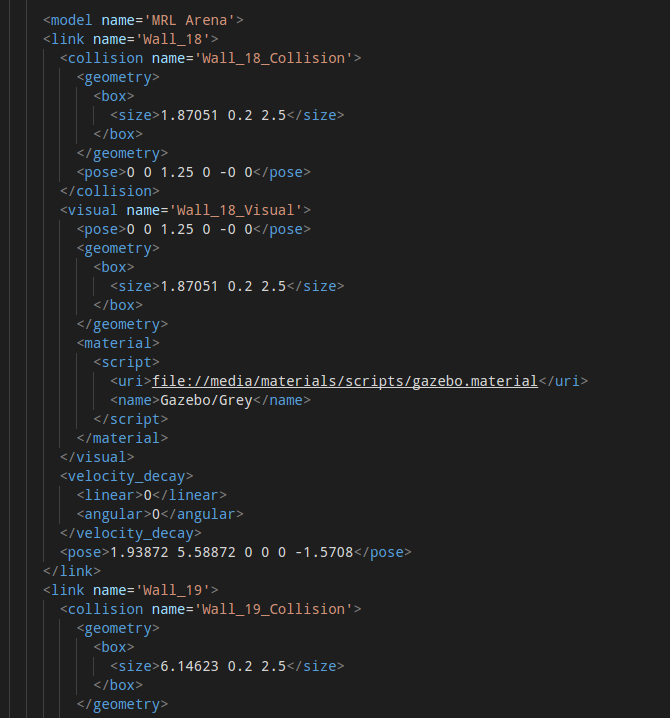
\includegraphics[width=0.7\linewidth, height=0.2\textheight]{figures/world_walls}
        \caption{The simple indoor URDF file}
        \label{fig:small_indoor}
    \end{minipage}%
    \begin{minipage}{0.5\textwidth}
        \centering
        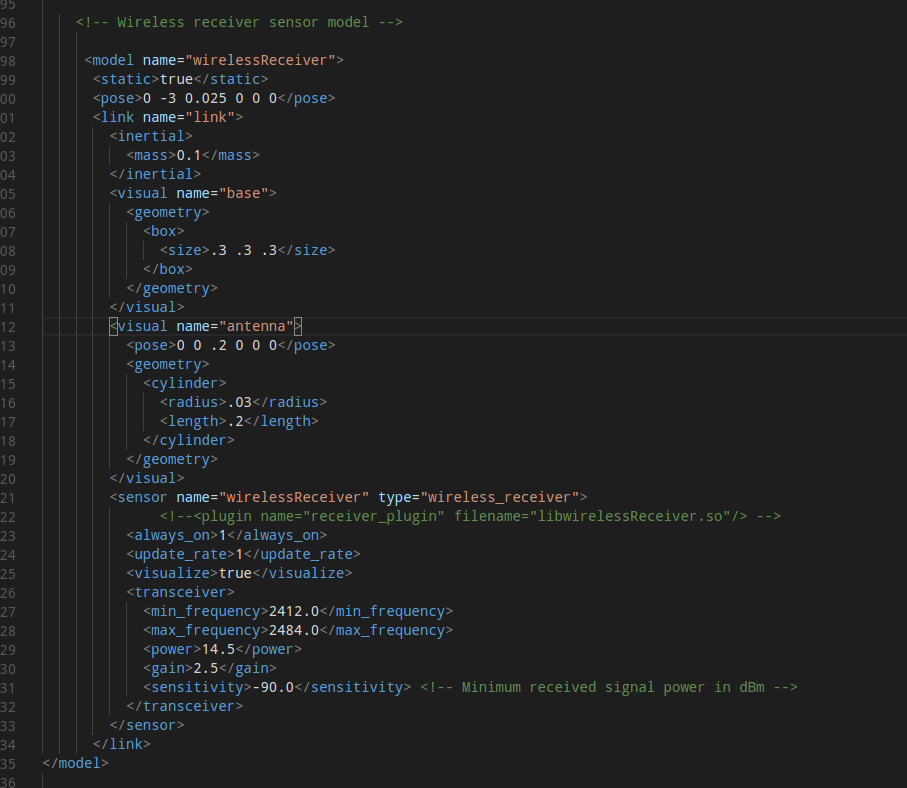
\includegraphics[width=1\linewidth, height=0.2\textheight]{figures/WirelessTransmitter}
        \caption{Details of the Wireless sensor model within the same URDF indoor model file}
        \label{fig:wireless_trans}
    \end{minipage}
 \end{figure}

Ones the small indoor model has been created, the pre-installed mapping algorithms provide by ROS, $Gmapping$ and $Amcl$ have to be tested. It is always good practice to download and build the packages from source when developers want to modify the files and adjust the internal parameters. The husky robot package together with the slam-gmapping one has been cloned from source, as seen in Figure \ref{fig:husky_str}

\begin{figure}[!htb]
	\center
	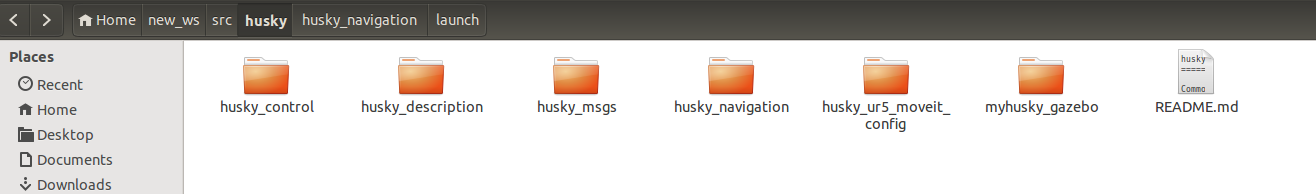
\includegraphics[width=0.9\textwidth]{figures/husky_pkg_struct.png}
	\caption{The husky package structure}
	\label{fig:husky_str}
\end{figure}

The husky robot package consists of the following subpackages, and tuneable parameters:
\begin{itemize}
\item husky{\_}description: contains meshes and urdf files that assemble the husky robot. Inside the urdf folder (not visible in this picture) all the husky robot properties are built using a special type of file called the $Xacro$ file, which is a more compact version of the URDF file. A proper and detailed documentation can be found under [2]. As like for the world model of Figure \ref{fig:small_indoor}, an URDF file contains the robot components as link tags, and additionally joint tags define how the components have to be linked together. Most of the parameters that we find here are:
\begin{itemize}
\item Height, lenght and width of the single robot components
\item Inertial values for the 6 degree of freedom
\item Sensors main parameters, if present. This is actually of importance for our case, hence the laser LIDAR Sick Navi contained in the Gazebo standard sensors for husky, have the following parameters:
\begin{itemize}
\item Update rate: frequency in $Hz$ for the sensor update
\item Min and Max angle: self explaining in $rad$. NOTE: this has been modified to have a 360 deg angle all around the robot, as prescribed in the paper of [3], which is the first method to be implemented.
\item Min and Max range: the smallest and the longest distance that the sensor can measure, expres in $meters$
\end{itemize}
\end{itemize}

\item husky{\_}navigation: here is were the $Gmapping$ and $amcl$ algorithms are fired, together with their parameters. The single parameters sets are seen in Figure \ref{fig:amcl_param}, the way to be used will be explained later on while talking on the algorithm implementation. Additinally, inside the navigation folder, the map folder contains the stored map after the $Gmapping$ runs, in a .png a .config file. For the small indoor the map has been created. It is visible in Figure \ref{fig:myamcl_map} that there are no particular distorsions and the filter works well.

\item myhusky{\_}gazebo: this is a personal created package, containing the self-made MRL Arena.world file and the launch files needed to fire the simulation over the Gazebo node.
\end{itemize}

\begin{figure}[!htb]
    \centering
    \begin{minipage}{.5\textwidth}
        \centering
        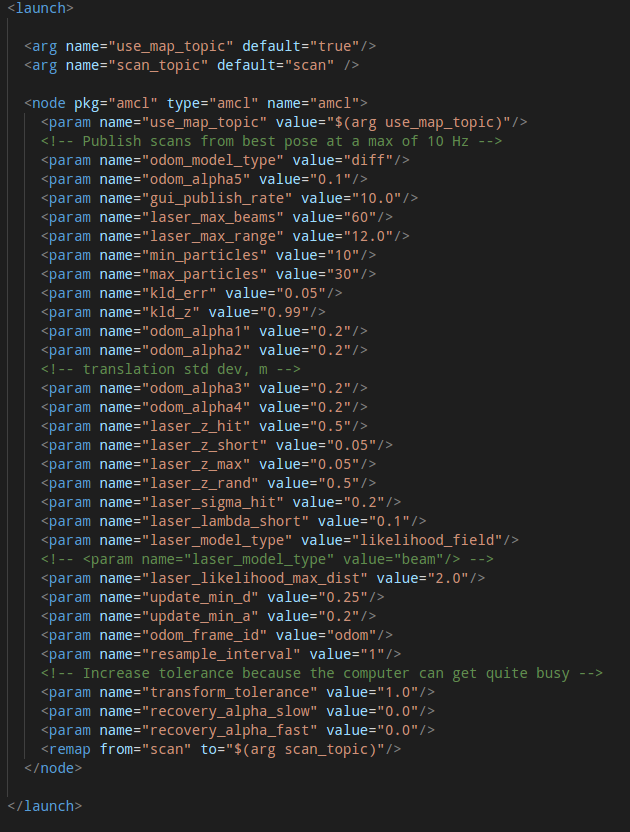
\includegraphics[width=0.7\linewidth, height=0.2\textheight]{figures/amcl_param}
        \caption{The $amcl$ tunable parameters}
        \label{fig:amcl_param}
    \end{minipage}%
    \begin{minipage}{0.5\textwidth}
        \centering
        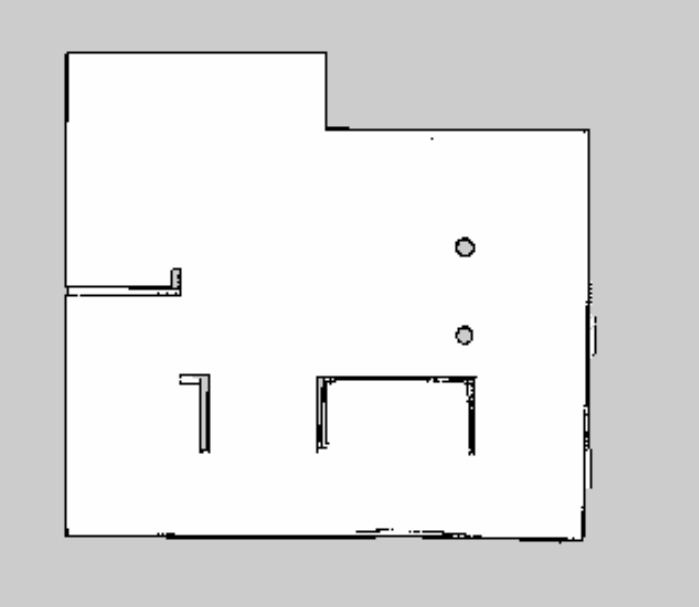
\includegraphics[width=0.7\linewidth, height=0.2\textheight]{figures/my_amcl_gmapping}
        \caption{Result of the Gmapping for the simple indoor environment}
        \label{fig:myamcl_map}
    \end{minipage}
 \end{figure}

So far, so good, and the husky model is now ready to be prepared and implement the approach described on [3]. To do so, the localization and navigation algorithm has been summarized with the main actions to take in the following pseudocode:

\begin{algorithm}[!h]
   \caption{Kirsch, Rohig algorithm}
    \begin{algorithmic}[1]
    	\State $St-1 = St$
        \For{$i = 1$ to $N$} \Comment{With N the number of particles in the filter set by maxparticle parameter}
            \State $Spread $ $particles$ $in$ $the$ $anchorbox$ $with$ $equations$ $1)$ $and$ $2)$ $of$ $[3]$ \Comment{This step is called $Global$ $Localization$}
            
            \State $xt[n] = p(xt|xt-1,ut)$ \Comment{Motion update - sample the particles from the motion update of the robot and move forward to estimate the error model functions}
            
        	\State $wt[n] = p(dnanoLOC|si)*p(dlaser|si)$ \Comment{Measurement update - si are the particles set with i the i-th index}
        	\State $St = St + <xt,wt>$ \Comment{add the state and weight to the total state space}
        	
        	\State $Perform$ $resampling$
        \EndFor
    \State $Return$ $St$

\end{algorithmic}
\end{algorithm}

We want to take advantage of the amcl node of ROS while making our personal algorithm implementation. To do so, we have to create our own node, communicating with the amcl one and getting the data that we need to perform the "personal algorithm" implementation. The second thing, is to modify the parameters of the amcl on the base of the actual performance during the simulation. The values of such parameters needs to be found empirically, even if for some of them rules exists. Additinally, the $move$ $base$, and inside of it the $local$ and $global$ $costmap$ parameters shoudl also be tuned. 

The number of parameters for the amcl, move base, local and global costmap is huge, so I am not going to describe them all. It is possible to define a detailed explanation of them at this reference [4]. In [4] there is a detailed explanation on how to tune them, and the approach really depends on the specific environment, as already cited.
In Figure \ref{fig:active_locnode} the overall vision of the nodes and topics communication is visible. This figure is actually taken from [4], but the actual personal one is pretty similar, just instead of a real robot, here called /volksbot, we use the informations from Gazebo to write on topics such as the $odometry$. Our "self-made" node wants from the amcl (node are the ellipses) informations on the global position of the robot in the environment. However, to perform a good global localization, the robot has to partially move, hence it has to publish data on the move base node, via move{\_}base/action{\_}topics. If the move base receives a new goal, it plans a path from the current pose of the robot to the goal pose. This global plan will be calculated using the Dijkstra algorithm. The planning of the global path is based on the information of the global costmap, which forces the planned path away from obstacles. The global plan will only change, if the local path planner notifies that an obstacle is in front of the robot or the global map changes (just by using the move base in conjunction with $GMapping$). The local path planner determines the velocity commands to execute the navigation, based on its local
costmap, which also detects obstacles in the environment.

The output it is written on the map topic, that progressively is built by the filter itself. 

\begin{figure}[!htb]
	\center
	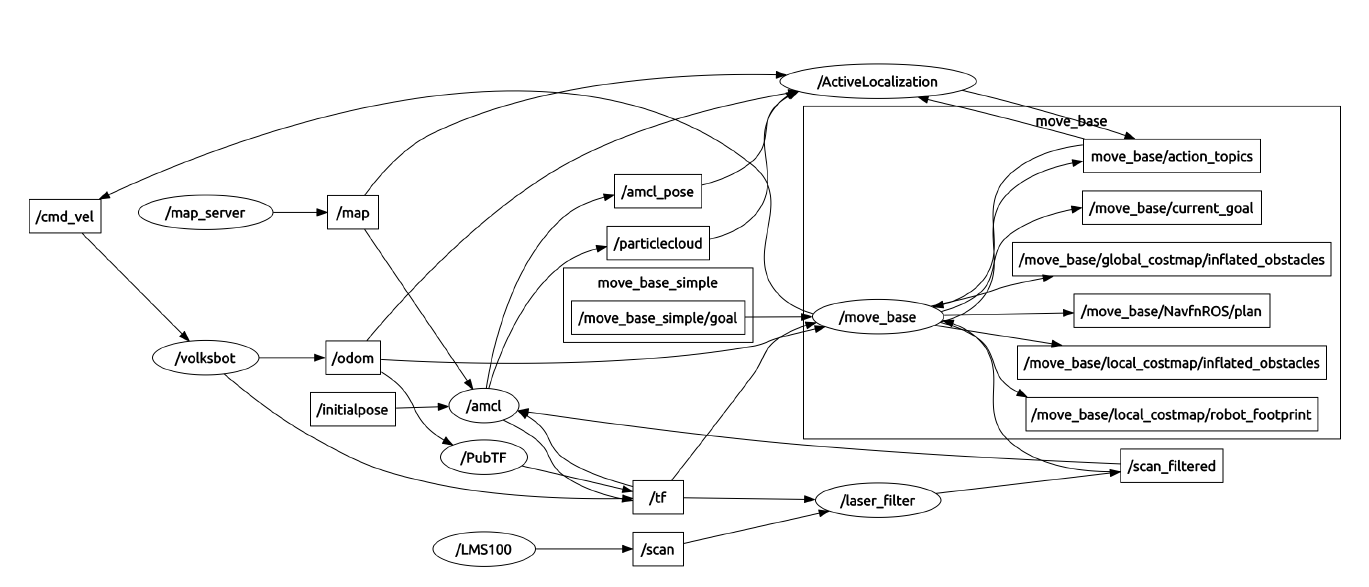
\includegraphics[width=1\textwidth]{figures/active_localization_node.png}
	\caption{An example of an active localization node}
	\label{fig:active_locnode}
\end{figure}

Answering to question 3) the deliverable is an algorithm that implement the pseudocode above, and that can be validated using the validation procedure. 

The validation answers the question number 4): first the algorithm has to be validated in close loop, to avoid map distorsions. Then an open loop manouvre is performed, that according to [5] is the typical path for indoor AGV, and recognized to be one of the toughest paths for the industrial reality. 

\section{Questions}

The questions are not specific but of general way, since you are probably not dealing with the same things: 
\begin{enumerate}
\item The first big question is more on a your opinion on the way I tackle the problem, so, if you had to do the same, how would you have done it?
\item Do you thing the creation of an additional node "The Active Localization" implementing the pseudocode in page 4 is a good strategy? The Amcl node already works, I can see the robot moving, the particles being spread, however the src code of the filter is not visible and I don´t know a way of controlling it.

We will discuss more thing during the meeting, I am actually curious to know your opinion.

\end{enumerate}

\section{Reference}

[1] J. Santos, D. Portugal, R. Rocha. An evaluation of 2D SLAM Techniques Available in Robot Operating System.

[2] http://wiki.ros.org/urdf/Tutorials/Using Xacro to Clean Up a URDF File

[3] Kirsch, C. and C.Rhig (2011). Global localization and position tracking of an automated guided vehicle.

[4] Sebastian Gangl, Robotic exploration for mapping and change detection. Pdf is available under Dropbox/Abschlussarbeit/PEM/Literature/LiteratureResearch/Thesis

[5] Investigating Simultaneous Localization and Mapping for AGV systems, A. Palsson, M. Smedberg

\end{document}






% == TABLE ==
%begin{table}[h!]
 % \centering
  %\caption{Caption for the table.}
 % \label{tab:table1}
 % \begin{tabular}{ccc}
 %   \toprule
  %  Some & actual & content\\
   % \midrule
   % prettifies & the & content\\
   % as & well & as\\
  %  using & the & booktabs package\\
  %   \bottomrule
  %\end{tabular}
%\end{table}